% ==============================================================================
% 6. PHÂN TÍCH KHÁM PHÁ DỮ LIỆU (EDA)
% ==============================================================================
\needspace{0.3\textheight}
\section{Phân tích khám phá dữ liệu (EDA)}
\label{sec:eda}

\textbf{Quy ước phân tích.}
\begin{itemize}
  \item Mọi thống kê được tách theo sáu nhóm: train, val, test của bộ chính (phân phối tự nhiên), pilot, tầng điểm cao và tầng ngẫu nhiên của ảnh bổ sung. Các kết quả gộp nhiều nhóm đều được ghi chú rõ.
  \item Nhãn val/test chỉ dùng để mô tả. Không có lựa chọn hay ngưỡng nào trong báo cáo được xác định dựa trên nhãn val/test.
  \item Khoảng tin cậy 95\% của tỉ lệ là khoảng Wilson~\cite{wilson1927interval}, giả định các ảnh độc lập. Do ảnh cùng đường có xu hướng giống nhau, khoảng thực tế rộng hơn; vì vậy các so sánh quan trọng có thêm khoảng \emph{bootstrap theo đường} (lấy mẫu lại theo nguyên tuyến đường), riêng với val (3 đường) và test (4 đường) chỉ có giá trị tham khảo.
  \item Mọi số liệu và hình trong mục này do ba script EDA của nhóm sinh ra, không nhập thủ công (phụ lục~\ref{sec:trace}).
\end{itemize}

% ------------------------------------------------------------------------------
\subsection{Thống kê mô tả}
\label{sec:eda-desc}

\subsubsection*{Số mẫu, số thuộc tính, tỉ lệ thiếu}

Bảng~\ref{tab:inventory} thống kê số dòng, số cột và dữ liệu thiếu của từng bảng dữ liệu.

\begin{table}[H]
\centering
\caption{Các bảng dữ liệu: số dòng, số cột, dữ liệu thiếu}
\label{tab:inventory}
\begin{tabularx}{\textwidth}{>{\raggedright\arraybackslash}p{0.33\linewidth} r r L}
\toprule
\textbf{Bảng} & \textbf{Dòng} & \textbf{Cột} & \textbf{Dữ liệu thiếu} \\
\midrule
Nhãn bộ chính và pilot & 3.149 & 8 & Chỉ cột lý do: thiếu ở 2.114 dòng, trong đó 1.833 dòng là nhãn 0/1 (không có lý do theo thiết kế) và \textbf{281 ảnh \lab{I} không có lý do} \\
Nhãn ảnh bổ sung & 2.000 & 11 & Chỉ cột lý do: 1.403 dòng, trong đó 7 ảnh \lab{I} không có lý do \\
Manifest bộ chính & 2.999 & 21 & Không thiếu ô nào \\
Manifest pilot & 150 & 21 & Không thiếu ô nào (không có cột nhóm vị trí) \\
Manifest ảnh bổ sung & 2.000 & 25 & Không thiếu ô nào \\
Từng lượt gán, bộ chính & 4.435 & 13 & Lý do, loại vật cản, ghi chú: thiếu theo thiết kế (không bắt buộc) \\
Từng lượt gán, ảnh bổ sung & 2.000 & 13 & Như trên \\
\bottomrule
\end{tabularx}
\end{table}

\begin{itemize}
  \item \textbf{Thuộc tính.} Mỗi ảnh có 1 nhãn và khoảng 20 thuộc tính metadata, gồm 7 thuộc tính số (vĩ độ, kinh độ, độ sáng ảnh $360^\circ$, khoảng cách tới tim đường, hướng di chuyển của xe, góc cắt, và điểm của bộ chọn ảnh đối với ảnh bổ sung); các thuộc tính còn lại là thuộc tính phân loại hoặc định danh (đường, tập, tài khoản chụp, chuỗi ảnh, thời gian chụp, tầng lấy mẫu, nguồn nhãn). Đầu vào của mô hình chỉ là ảnh; metadata được dùng để chia tập, truy nguồn và kiểm tra.
  \item \textbf{Metadata không thiếu ô nào} trên toàn bộ 5.149 ảnh, vì ảnh thiếu tọa độ hoặc hướng di chuyển không gắn được vào đường nên không thể được chọn.
  \item \textbf{281 ảnh \lab{I} của bộ chính và pilot không ghi lý do}, gồm 162 ảnh có nhãn sau phân xử, 63 ảnh pilot (được xem lại theo v1 nhưng không ghi lý do), 55 ảnh mà hai người cùng chọn \lab{I} nhưng khác lý do, và 1 ảnh chỉ có một người gán. Vì vậy, thống kê lý do chỉ tính trên 1.035/1.253 ảnh \lab{I} của bộ chính. Nhãn chính không bị ảnh hưởng.
\end{itemize}

\subsubsection*{Thống kê cơ bản của các biến số}

Bảng~\ref{tab:desc} và hình~\ref{fig:desc} mô tả hai biến số chính theo từng nhóm; bảng~\ref{tab:desc2} mô tả các biến số còn lại.

\begin{table}[H]
\centering
\caption{Thống kê mô tả hai biến số chính của metadata, theo nhóm}
\label{tab:desc}
\small\setlength{\tabcolsep}{4pt}
\begin{tabularx}{\textwidth}{>{\raggedright\arraybackslash}p{0.2\linewidth} r R R R R R R}
\toprule
\textbf{Nhóm} & \textbf{n} & \textbf{Trung bình} & \textbf{Trung vị} & \textbf{Phương sai} & \textbf{Nhỏ nhất} & \textbf{Lớn nhất} & \textbf{IQR} \\
\midrule
\multicolumn{8}{l}{\emph{Độ sáng ảnh $360^\circ$ (trung bình nửa trên, thang 0--255)}} \\
Bộ chính, train & 1.839 & 166,8 & 171,0 & 448,6 & 94 & 231 & 27,0 \\
Bộ chính, val & 486 & 154,5 & 158,5 & 468,9 & 91 & 201 & 32,0 \\
Bộ chính, test & 674 & 169,4 & 171,0 & 564,2 & 91 & 249 & 26,8 \\
Pilot & 150 & 169,2 & 173,5 & 573,5 & 94 & 236 & 27,0 \\
Ảnh bổ sung, tầng điểm cao & 1.400 & 172,0 & 176,0 & 366,8 & 91 & 239 & 19,0 \\
Ảnh bổ sung, tầng ngẫu nhiên & 600 & 172,7 & 176,0 & 377,9 & 94 & 238 & 22,3 \\
\midrule
\multicolumn{8}{l}{\emph{Khoảng cách từ vị trí chụp tới tim đường (m)}} \\
Bộ chính, train & 1.839 & 3,70 & 3,0 & 9,67 & 0,0 & 20,0 & 3,40 \\
Bộ chính, val & 486 & 3,46 & 3,1 & 8,53 & 0,0 & 18,4 & 3,08 \\
Bộ chính, test & 674 & 3,54 & 2,9 & 9,48 & 0,0 & 19,6 & 3,70 \\
Pilot & 150 & 3,45 & 2,7 & 7,98 & 0,0 & 17,0 & 3,58 \\
Ảnh bổ sung, tầng điểm cao & 1.400 & 2,87 & 2,2 & 6,81 & 0,0 & 19,9 & 2,70 \\
Ảnh bổ sung, tầng ngẫu nhiên & 600 & 2,96 & 2,3 & 7,24 & 0,0 & 19,8 & 2,90 \\
\bottomrule
\end{tabularx}
\note{IQR: khoảng tứ phân vị (hiệu giữa tứ phân vị thứ ba và tứ phân vị thứ nhất).}
\end{table}

\begin{figure}[H]
\centering
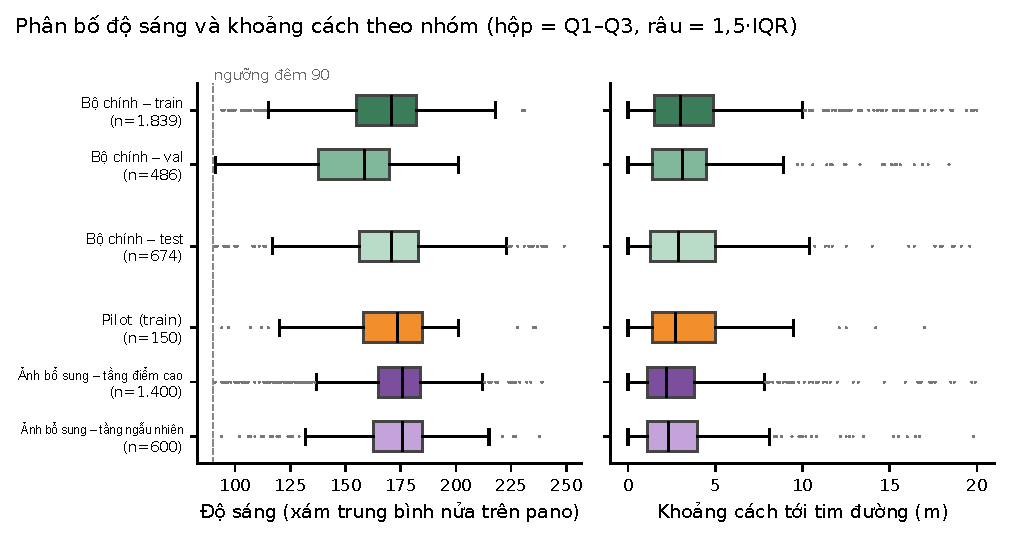
\includegraphics[width=0.95\textwidth]{tab_fig4_brightness_dist_boxplots.pdf}
\caption{Phân bố độ sáng ảnh $360^\circ$ và khoảng cách tới tim đường theo nhóm}
\label{fig:desc}
\end{figure}

\begin{table}[H]
\centering
\caption{Thống kê mô tả các biến số còn lại của metadata}
\label{tab:desc2}
\footnotesize\setlength{\tabcolsep}{3pt}
\begin{tabularx}{\textwidth}{>{\raggedright\arraybackslash}p{0.17\linewidth} r R R R R R R}
\toprule
\textbf{Nhóm} & \textbf{n} & \textbf{Trung bình} & \textbf{Trung vị} & \textbf{Phương sai} & \textbf{Nhỏ nhất} & \textbf{Lớn nhất} & \textbf{IQR} \\
\midrule
\multicolumn{8}{l}{\emph{Vĩ độ ($^\circ$ Bắc)}} \\
Bộ chính, gộp & 2.999 & 10,7751 & 10,7757 & $2{,}7\cdot10^{-4}$ & 10,7501 & 10,8149 & 0,0274 \\
Ảnh bổ sung, gộp & 2.000 & 10,7812 & 10,7860 & $4{,}3\cdot10^{-4}$ & 10,7450 & 10,8150 & 0,0359 \\
\multicolumn{8}{l}{\emph{Kinh độ ($^\circ$ Đông)}} \\
Bộ chính, gộp & 2.999 & 106,6792 & 106,6813 & $2{,}3\cdot10^{-4}$ & 106,6500 & 106,7059 & 0,0285 \\
Ảnh bổ sung, gộp & 2.000 & 106,6813 & 106,6813 & $3{,}1\cdot10^{-4}$ & 106,6500 & 106,7234 & 0,0291 \\
\multicolumn{8}{l}{\emph{Hướng di chuyển của xe ($^\circ$, 0 = hướng Bắc)}} \\
Bộ chính, gộp & 2.999 & 166,5 & 164,7 & 10.589,6 & 0,0 & 360,0 & 193,3 \\
Ảnh bổ sung, gộp & 2.000 & 178,0 & 167,5 & 10.050,7 & 0,1 & 359,6 & 180,3 \\
\multicolumn{8}{l}{\emph{Điểm của bộ chọn ảnh (chỉ có ở ảnh bổ sung, thang 0--1)}} \\
Tầng điểm cao & 1.400 & 0,799 & 0,798 & 0,012 & 0,610 & 0,996 & 0,191 \\
Tầng ngẫu nhiên & 600 & 0,231 & 0,188 & 0,032 & 0,001 & 0,607 & 0,286 \\
\multicolumn{8}{l}{\emph{Thời gian gán một ảnh (giây, tính theo lượt gán)}} \\
Bộ chính & 4.435 & 51,5 & 3,7 & 2.285.741 & 0,5 & 77.451 & 6,9 \\
Ảnh bổ sung & 2.000 & 13,9 & 4,5 & 24.475 & 0,9 & 6.678 & 5,3 \\
\bottomrule
\end{tabularx}
\note{Góc cắt không được đưa vào bảng vì là hằng số ($60^\circ$ về bên phải) với mọi ảnh.}
\end{table}

\begin{itemize}
  \item \textbf{Độ sáng} (bảng~\ref{tab:desc}, hình~\ref{fig:desc}). Không ảnh nào có độ sáng dưới ngưỡng lọc ảnh đêm (nhỏ nhất là 91). Ảnh tập val tối hơn các nhóm khác (trung vị 158,5 so với 171); do val chỉ có 3 đường, đây có thể là đặc điểm riêng của ba đường này.
  \item \textbf{Khoảng cách tới tim đường} bị giới hạn trên ở 20 m theo quy tắc gắn đường. Ảnh bổ sung gần tim đường hơn (trung vị 2,2 m so với 3,0 m), phù hợp với việc 71\% ảnh bổ sung đến từ đường nhỏ.
  \item \textbf{Tọa độ} (bảng~\ref{tab:desc2}) nằm trong khung nghiên cứu, trừ 2 ảnh bổ sung lệch ra ngoài dưới 4 m (mục~\ref{sec:eda-quality}). Ảnh bổ sung phân tán rộng hơn bộ chính (IQR của vĩ độ là 0,0359 so với 0,0274) vì đến từ 75 đường thay vì 17 đường.
  \item \textbf{Hướng di chuyển của xe} trải đều trên toàn dải 0--$360^\circ$ (IQR xấp xỉ $190^\circ$), không tập trung vào một hướng. Thuộc tính này chỉ được dùng để gắn ảnh vào đường và để cắt ảnh về phía bên phải xe.
  \item \textbf{Điểm của bộ chọn ảnh} (chỉ có ở ảnh bổ sung): tầng điểm cao có trung vị 0,80 (0,61--1,00), tầng ngẫu nhiên có trung vị 0,19 (0,00--0,61).
  \item \textbf{Thời gian gán một ảnh} lệch phải rất mạnh: trung vị là 3,7 giây (bộ chính, 4.435 lượt) và 4,5 giây (ảnh bổ sung), trong khi giá trị lớn nhất lên tới 77.451 giây do một số tác vụ bị để mở. Vì vậy, trung vị là thước đo phù hợp hơn trung bình. Thời gian gán của pilot \textbf{chưa được đo} trong báo cáo này.
\end{itemize}

\subsubsection*{Phân bố theo thuộc tính phân loại}

Hình~\ref{fig:year} và bảng~\ref{tab:month} trình bày phân bố ảnh theo tài khoản chụp, năm chụp và tháng chụp.

\begin{figure}[H]
\centering
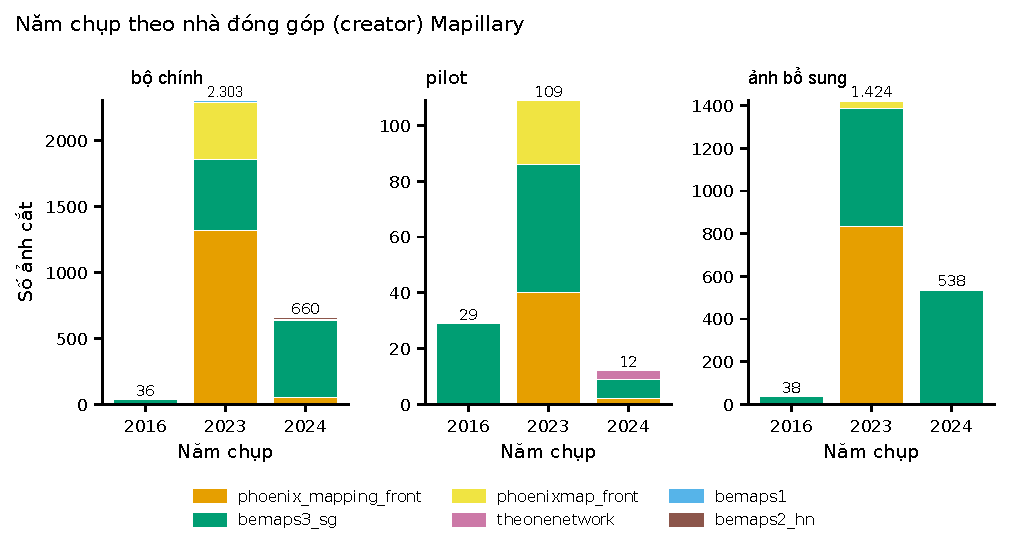
\includegraphics[width=0.95\textwidth]{tab_fig5_year_creator.pdf}
\caption{Số ảnh theo năm chụp và tài khoản chụp}
\label{fig:year}
\end{figure}

\begin{table}[H]
\centering
\caption{Số ảnh theo tháng chụp (theo dấu thời gian của Mapillary)}
\label{tab:month}
\setlength{\tabcolsep}{3.5pt}
\begin{tabular}{l rrrrrrrrrrrr r}
\toprule
\textbf{Tháng} & 1 & 2 & 3 & 4 & 5 & 6 & 7 & 8 & 9 & 10 & 11 & 12 & \textbf{Tổng} \\
\midrule
Bộ chính & 299 & 114 & 0 & 552 & 677 & 234 & 0 & 244 & 54 & 321 & 303 & 201 & 2.999 \\
Ảnh bổ sung & 146 & 204 & 53 & 93 & 461 & 286 & 0 & 55 & 87 & 96 & 342 & 177 & 2.000 \\
\bottomrule
\end{tabular}
\end{table}

\begin{itemize}
  \item \textbf{Tài khoản chụp} (hình~\ref{fig:year}). Hai tài khoản \lab{bemaps3\_sg} và \lab{phoenix\_mapping\_front} chiếm 84\% bộ chính (1.153 và 1.370 trên 2.999 ảnh) và 98\% ảnh bổ sung. Do đó, dữ liệu đến từ rất ít loại thiết bị và cách gắn camera.
  \item \textbf{Năm chụp.} Ở bộ chính, năm 2023 có 2.303 ảnh, năm 2024 có 660 ảnh và năm 2016 có 36 ảnh. Toàn bộ 103 ảnh ghi năm 2016 (trên cả ba phần dữ liệu) đều thuộc tài khoản \lab{bemaps3\_sg} và cùng ghi ngày 01/01/2016; nhiều khả năng đây là ngày mặc định, nên năm 2016 \textbf{không đáng tin cậy}.
  \item \textbf{Tháng chụp} (bảng~\ref{tab:month}). Ảnh được chụp trong 10 tháng khác nhau (bộ chính) và 11 tháng khác nhau (ảnh bổ sung), không có ảnh nào vào tháng 7; ảnh bộ chính tập trung vào tháng 4--5 (41\%). Tháng 1 bao gồm cả các ảnh mang ngày mặc định 01/01/2016.
  \item \textbf{Giờ chụp} trải khắp các khung giờ trong ngày nhưng không đáng tin cậy: ở bộ chính, 1.080/2.999 ảnh (36\%) ghi giờ từ 18 giờ tới trước 6 giờ sáng (ở ảnh bổ sung là 762/2.000, tức 38\%), trong khi mọi ảnh được giữ lại đều vượt ngưỡng độ sáng của bộ lọc ảnh đêm. Vì vậy, giờ chụp không được dùng để lọc ảnh (mục~\ref{sec:cleaning}).
  \item \textbf{Số ảnh mỗi đường.} Bộ chính có 17 đường, mỗi đường 86--348 ảnh (trung vị 150); ảnh bổ sung có 75 đường, mỗi đường 6--157 ảnh (trung vị 21). Hai đường ven kênh Hoàng Sa và Trường Sa\#0 đóng góp 274 ảnh bổ sung (14\%). Hai đường này từng bị loại khỏi bộ chính vì vỉa hè chủ yếu nằm ở một phía và có ít người đi bộ (bước 4, bảng~\ref{tab:steps}). Tuy nhiên, đợt bổ sung chỉ xếp hạng đường theo điểm của bộ chọn ảnh và không áp dụng lại tiêu chí này: hai đường đứng hạng 49 và 56 trong 75 đường, và do có chiều dài lớn nên đóng góp nhiều ảnh. Hai đường này chỉ thuộc train nên không ảnh hưởng tới val/test, nhưng làm tăng tỉ lệ cảnh ven kênh trong train.
\end{itemize}

% ------------------------------------------------------------------------------
\subsection{Phân tích phân bố nhãn}
\label{sec:eda-labels}

Mục này xét mức mất cân bằng giữa các lớp, tỉ lệ từng lớp theo nhóm, thành phần nhãn của tập train sau khi bổ sung, và sự khác biệt theo đường, theo loại vật cản và theo người gán.

\begin{figure}[H]
\centering
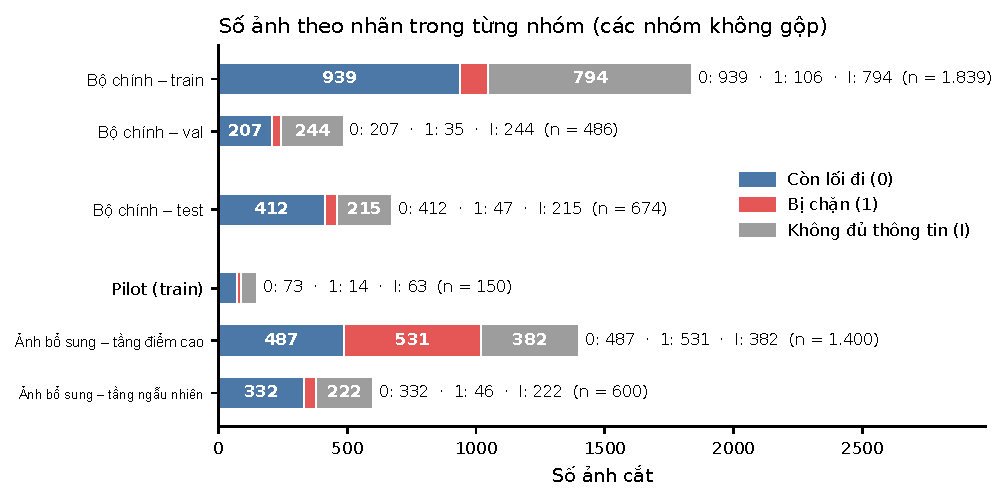
\includegraphics[width=0.95\textwidth]{tab_fig1_label_counts_by_group.pdf}
\caption{Số ảnh theo nhãn trong từng nhóm}
\label{fig:labels}
\end{figure}

\begin{table}[H]
\centering
\caption{Tỉ lệ \lab{Bị chặn} và \lab{Không đủ thông tin} theo nhóm, khoảng tin cậy 95\%}
\label{tab:labels}
\begin{tabularx}{\textwidth}{>{\raggedright\arraybackslash}p{0.2\linewidth} r >{\raggedright\arraybackslash}p{0.2\linewidth} >{\raggedright\arraybackslash}p{0.14\linewidth} r r}
\toprule
\textbf{Nhóm} & \textbf{Ảnh} & \textbf{Bị chặn / hợp lệ [Wilson]} & \textbf{Bootstrap theo đường} & \textbf{Tỉ lệ I} & \textbf{0 : 1} \\
\midrule
Bộ chính, train & 1.839 & 106/1.045 = 10,1\% [8,5; 12,1] & [7,9; 14,1] & 43,2\% & 8,9 \\
Bộ chính, val & 486 & 35/242 = 14,5\% [10,6; 19,4] & [8,2; 19,2] & 50,2\% & 5,9 \\
Bộ chính, test & 674 & 47/459 = 10,2\% [7,8; 13,4] & [5,7; 18,7] & 31,9\% & 8,8 \\
\emph{Bộ chính, gộp} & 2.999 & 188/1.746 = 10,8\% [9,4; 12,3] & [8,7; 13,9] & 41,8\% & 8,3 \\
\midrule
Pilot & 150 & 14/87 = 16,1\% [9,8; 25,2] & [10,0; 18,4] & 42,0\% & 5,2 \\
Ảnh bổ sung, tầng điểm cao & 1.400 & 531/1.018 = 52,2\% [49,1; 55,2] & [47,8; 56,6] & 27,3\% & 0,9 \\
Ảnh bổ sung, tầng ngẫu nhiên & 600 & 46/378 = 12,2\% [9,2; 15,9] & [8,9; 15,3] & 37,0\% & 7,2 \\
\bottomrule
\end{tabularx}
\note{Ảnh hợp lệ là ảnh có nhãn 0 hoặc 1. Bootstrap theo đường: 1.000 lần lấy mẫu lại.}
\end{table}

\begin{itemize}
  \item \textbf{Dữ liệu tự nhiên mất cân bằng mạnh} (hình~\ref{fig:labels}, bảng~\ref{tab:labels}): trong các ảnh hợp lệ của bộ chính, \lab{Còn lối đi} chiếm 89,2\% và \lab{Bị chặn} chiếm 10,8\%, tức cứ khoảng 8 ảnh \lab{Còn lối đi} mới có 1 ảnh \lab{Bị chặn}. Tính trên mọi ảnh, kể cả ảnh \lab{I}, tỉ lệ \lab{Bị chặn} là 6,3\% $[5{,}5;\,7{,}2]$.
  \item \textbf{Tỉ lệ ba lớp \lab{0} / \lab{1} / \lab{I} trên mọi ảnh:} bộ chính gộp 52,0 / 6,3 / 41,8\%; train 51,1 / 5,8 / 43,2\%; val 42,6 / 7,2 / 50,2\%; test 61,1 / 7,0 / 31,9\%; pilot 48,7 / 9,3 / 42,0\%; tầng điểm cao 34,8 / 37,9 / 27,3\%; tầng ngẫu nhiên 55,3 / 7,7 / 37,0\%. Trên toàn bộ dữ liệu: 47,6 / 15,1 / 37,3\%.
  \item \textbf{Khoảng tin cậy của tỉ lệ \lab{Bị chặn} ở ba tập chồng lên nhau} (tỉ lệ lần lượt là 10,1\%, 14,5\% và 10,2\%). Tuy nhiên, điều này chưa đủ để kết luận các tỉ lệ là tương đương.
  \item \textbf{Test chỉ có 47 mẫu dương, val có 35 mẫu dương.} Độ rộng khoảng bootstrap theo đường của test gấp xấp xỉ 2,3 lần độ rộng khoảng Wilson ($[5{,}7;\,18{,}7]$ so với $[7{,}8;\,13{,}4]$, tức 13,0 so với 5,6 điểm phần trăm), nên kết quả đánh giá mô hình trên test sẽ có sai số lớn.
  \item \textbf{Ảnh \lab{I} chiếm 32--50\%} tùy tập. Đây là hạn chế cố hữu của nguồn ảnh chụp từ xe.
  \item \textbf{Tỉ lệ ở pilot và tầng điểm cao không phản ánh phân phối tự nhiên:} tỉ lệ \lab{Bị chặn} của hai nhóm này (16,1\% và 52,2\%) là kết quả của cách lấy mẫu, không phải tỉ lệ thực tế ngoài đường.
  \item \textbf{Tầng ngẫu nhiên của ảnh bổ sung (12,2\%)} có tỉ lệ gần với bộ chính dù được lấy từ các đường khác; hai khoảng tin cậy chồng lên nhau.
\end{itemize}

\begin{figure}[H]
\centering
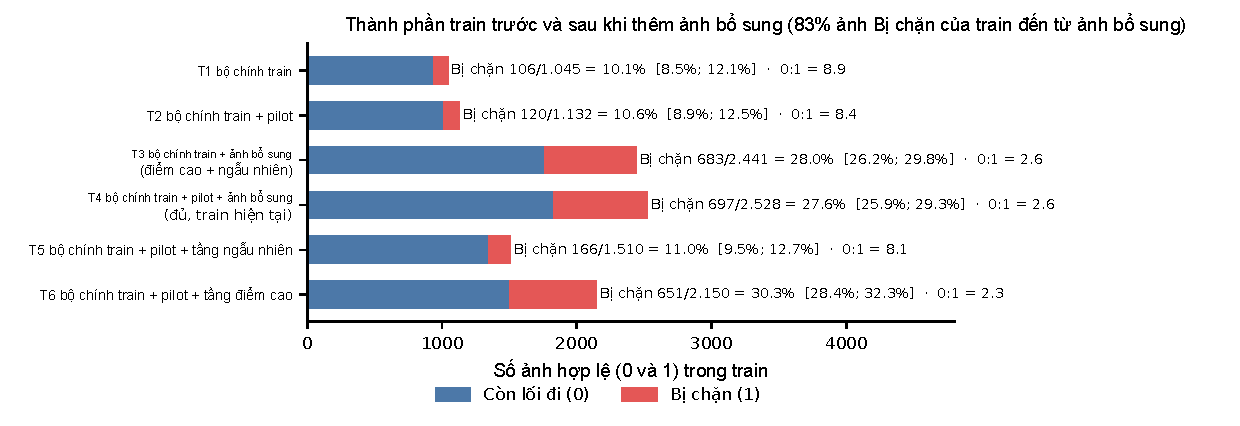
\includegraphics[width=\textwidth]{tab_fig10_train_composition.pdf}
\caption{Thành phần tập train trước và sau khi thêm pilot và ảnh bổ sung (chỉ tính ảnh hợp lệ)}
\label{fig:train}
\end{figure}

\textbf{Tập train sau khi bổ sung} (hình~\ref{fig:train}). Train hiện có 2.528 ảnh hợp lệ, trong đó 697 mẫu dương (27,6\%, tỉ lệ 0:1 là 2,6), so với 1.132 ảnh hợp lệ và 120 mẫu dương (10,6\%) trước khi bổ sung. 577 trong 697 mẫu dương (83\%) đến từ ảnh bổ sung. Hệ quả là phân phối nhãn của train khác với val/test (27,6\% so với khoảng 10--15\%); khi huấn luyện cần tính tới độ lệch này, đồng thời nên báo cáo thêm kết quả khi chỉ huấn luyện trên phần dữ liệu tự nhiên.

\begin{figure}[H]
\centering
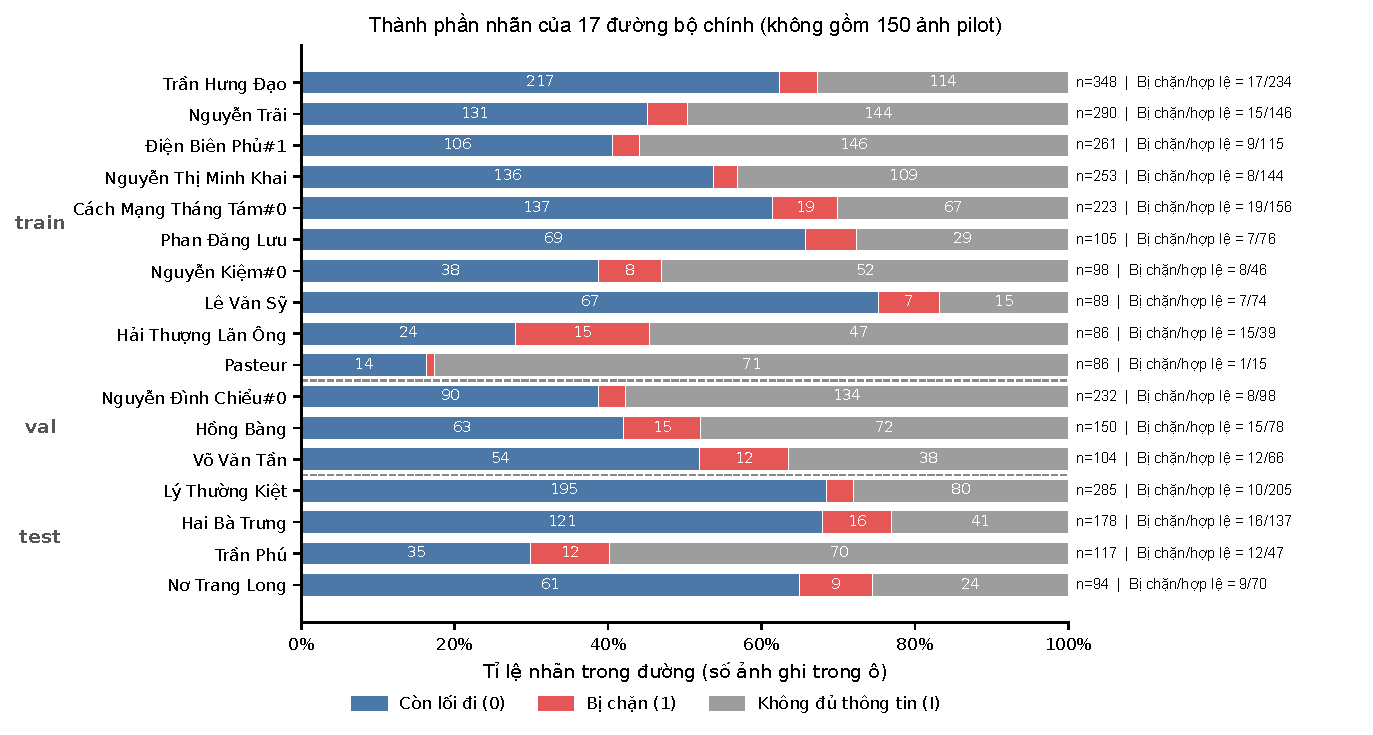
\includegraphics[width=\textwidth]{tab_fig3a_main_street_composition.pdf}
\caption{Thành phần nhãn của 17 đường thuộc bộ chính (không gồm pilot)}
\label{fig:streets}
\end{figure}

\textbf{Theo đường} (hình~\ref{fig:streets}). Tỉ lệ nhãn khác nhau đáng kể giữa các đường: tỉ lệ \lab{Bị chặn} trên ảnh hợp lệ dao động từ 4,9\% (Lý Thường Kiệt, 10/205) tới 38,5\% (Hải Thượng Lãn Ông, 15/39); tỉ lệ \lab{I} dao động từ 17\% (Lê Văn Sỹ) tới 83\% (Pasteur, đường một chiều). Ở ảnh bổ sung, trong 25 đường có ít nhất 20 ảnh hợp lệ, tỉ lệ \lab{Bị chặn} dao động từ 11,1\% (Bạch Đằng\#0, 4/36) tới 76,2\% (Ung Văn Khiêm, 16/21), trung vị 40,0\%; các tỉ lệ này gộp hai tầng nên chịu ảnh hưởng của cách chọn ảnh. Tuyến đường là thuộc tính có mức liên hệ với nhãn mạnh nhất (mục~\ref{sec:eda-rel}), vì vậy việc chia tập theo đường là cần thiết để tránh đánh giá quá lạc quan.

\begin{figure}[H]
\centering
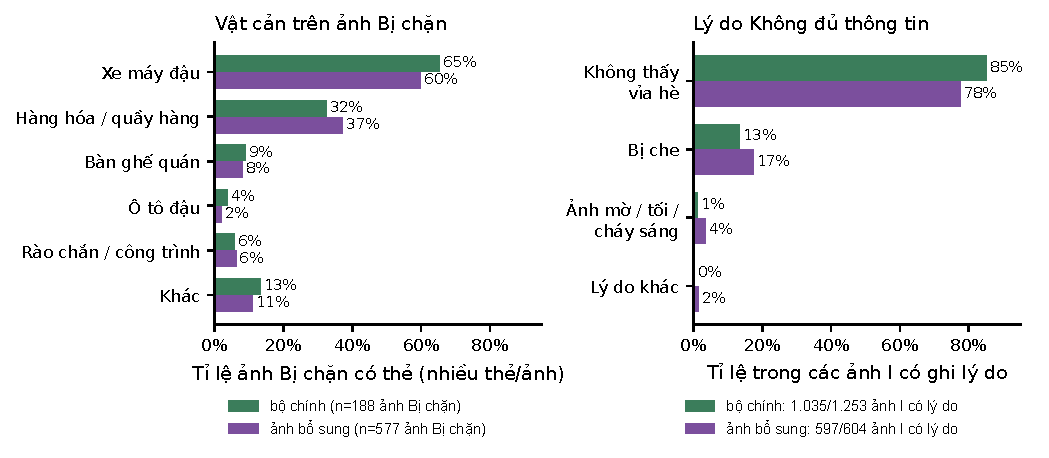
\includegraphics[width=0.95\textwidth]{tab_fig7_obstacles_reasons.pdf}
\caption{Loại vật cản trên ảnh \lab{Bị chặn} và lý do gán nhãn \lab{Không đủ thông tin}, bộ chính so với ảnh bổ sung}
\label{fig:obstacles}
\end{figure}

\textbf{Đa dạng của vật cản và lý do gán nhãn \lab{I}} (hình~\ref{fig:obstacles}).
\begin{itemize}
  \item Trên ảnh \lab{Bị chặn}, xe máy đậu là loại vật cản phổ biến nhất (bộ chính 123/188 ảnh, 65\%; ảnh bổ sung 346/577 ảnh, 60\%), tiếp theo là hàng hóa và quầy hàng (32\% và 37\%). Ô tô đậu hiếm gặp (4\% và 2\%). Một ảnh có thể có nhiều loại vật cản. Cơ cấu vật cản của hai phần dữ liệu khá tương đồng.
  \item Lý do gán \lab{I} chủ yếu là không thấy vỉa hè (bộ chính 880/1.035 ảnh có ghi lý do, 85\%; ảnh bổ sung 463/597 ảnh, 78\%), tiếp theo là vỉa hè bị che khuất. Ảnh mờ, tối hoặc cháy sáng chỉ có 12 và 21 ảnh.
  \item Thẻ vật cản là thông tin phụ, không bắt buộc: 13 ảnh \lab{Bị chặn} của bộ chính và 6 ảnh bổ sung không có thẻ nào. Thẻ vật cản của pilot \textbf{chưa được thống kê}.
\end{itemize}
\note{Thẻ vật cản của một ảnh là hợp của các thẻ từ những lượt gán nhãn 1 cho ảnh đó.}

\begin{figure}[H]
\centering
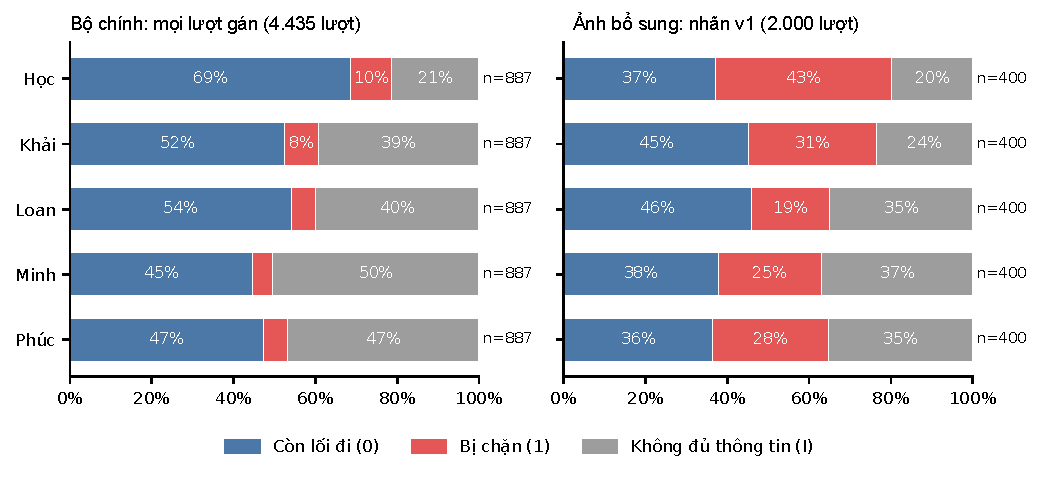
\includegraphics[width=0.95\textwidth]{tab_fig8_annotator_label_shares.pdf}
\caption{Tỉ lệ nhãn theo người gán; phần ảnh bổ sung dùng nhãn của từng người trước kiểm tra chéo}
\label{fig:annotators}
\end{figure}

\textbf{Theo người gán} (hình~\ref{fig:annotators}). Ở ảnh bổ sung, ảnh được chia ngẫu nhiên cho người gán nên chênh lệch giữa người gán gợi ý sự khác biệt trong cách gán, nhưng cần cho nhiều người cùng gán một mẫu ảnh để xác nhận: tỉ lệ \lab{Bị chặn} dao động từ 19\% (Loan) tới 43\% (Học). Ở bộ chính, mỗi người gán một phần ảnh khác nhau (hai người gán test, hai người gán val), nên tỉ lệ theo người gán bị lẫn với ảnh hưởng của tập và không so sánh trực tiếp được.

% ------------------------------------------------------------------------------
\subsection{Phân tích mối quan hệ giữa các thuộc tính}
\label{sec:eda-rel}

Đầu vào của mô hình là ảnh, không phải metadata. Mục này trả lời hai câu hỏi: các thuộc tính metadata có trùng lặp thông tin với nhau không, và có thuộc tính nào liên hệ với nhãn tới mức cần đề phòng mô hình học lối tắt (shortcut learning) không. Với biến số, mức liên hệ với nhãn được đo bằng AUC (diện tích dưới đường cong ROC; 0,5 nghĩa là không phân biệt được hai lớp); với biến phân loại, mức liên hệ được đo bằng Cramér's V hiệu chỉnh độ chệch.

\begin{figure}[H]
\centering
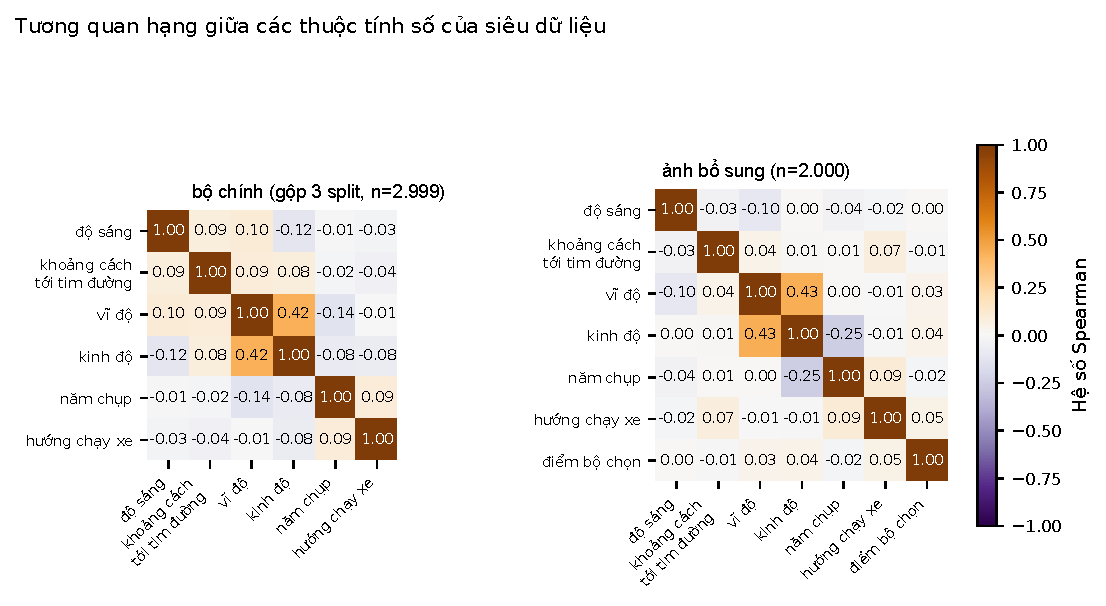
\includegraphics[width=0.95\textwidth]{tab_fig6_spearman_heatmap.pdf}
\caption{Tương quan hạng Spearman giữa các thuộc tính số của metadata}
\label{fig:spearman}
\end{figure}

\begin{itemize}
  \item \textbf{Tương quan} (hình~\ref{fig:spearman}). Cặp duy nhất có tương quan đáng kể là vĩ độ--kinh độ ($\rho = 0{,}42$ ở bộ chính, 0,43 ở ảnh bổ sung), do hình dạng khu vực nghiên cứu và hướng của các tuyến đường. Mọi cặp còn lại có $|\rho| \le 0{,}14$ ở bộ chính và $\le 0{,}25$ ở ảnh bổ sung.
  \item \textbf{Đa cộng tuyến.} Hệ số phóng đại phương sai (VIF) lớn nhất là 1,27 (vĩ độ) và 1,25 (kinh độ) ở bộ chính, do hai biến này tương quan với nhau; các biến khác đều dưới 1,1. Không thấy dấu hiệu đa cộng tuyến đáng kể giữa các biến được kiểm tra.
\end{itemize}

\begin{table}[H]
\centering
\caption{Liên hệ giữa thuộc tính và nhãn \lab{Bị chặn} so với \lab{Còn lối đi} (ảnh hợp lệ)}
\label{tab:assoc}
\begin{tabularx}{\textwidth}{>{\raggedright\arraybackslash}p{0.3\linewidth} L L}
\toprule
\textbf{Thuộc tính} & \textbf{Bộ chính, gộp (n = 1.746)} & \textbf{Ảnh bổ sung (n = 1.396)} \\
\midrule
\multicolumn{3}{l}{\emph{Biến số: AUC (0,5 = không phân biệt), khoảng bootstrap theo đường}} \\
Độ sáng ảnh $360^\circ$ & 0,53 [0,47; 0,59] & 0,49 [0,45; 0,53] \\
Khoảng cách tới tim đường & 0,54 [0,50; 0,58] & 0,46 [0,43; 0,49] \\
Vĩ độ & 0,45 [0,37; 0,52] & khoảng tin cậy chứa 0,5 \\
Kinh độ & 0,45 [0,35; 0,54] & khoảng tin cậy chứa 0,5 \\
Điểm của bộ chọn ảnh & không có & 0,78 [0,75; 0,81] \\
\midrule
\multicolumn{3}{l}{\emph{Biến phân loại: Cramér's V hiệu chỉnh độ chệch~\cite{bergsma2013cramer} (0 = không liên hệ)}} \\
Tuyến đường & 0,18 & 0,29 \\
Loại đường & 0,00 (chỉ 2 mức) & 0,14 [0,06; 0,24] \\
Tài khoản chụp & 0,00 & 0,03 \\
Năm chụp & 0,02 & 0,03 \\
\bottomrule
\end{tabularx}
\note{Giá trị $p$ của các kiểm định này được tính với giả định ảnh độc lập nên quá lạc quan; báo cáo chỉ dựa vào độ lớn hiệu ứng.}
\end{table}

\begin{itemize}
  \item \textbf{Tuyến đường là thuộc tính có mức liên hệ với nhãn mạnh nhất}, với cả \lab{Bị chặn} (V = 0,18) lẫn \lab{I} (V = 0,28 ở bộ chính). Đây là lý do chính để chia tập theo đường.
  \item \textbf{Loại đường} (theo phân loại của OSM) có liên hệ với nhãn ở ảnh bổ sung: trong tầng ngẫu nhiên, tỉ lệ \lab{Bị chặn} trên ảnh hợp lệ là 13,7\% ở đường nhánh (tertiary, 34/248) và 20\% ở đường khu dân cư (residential, 4/20), so với 7,0\% ở đường chính (primary, 3/43) và 7,5\% ở đường cấp hai (secondary, 5/67). Do cỡ mẫu các nhóm nhỏ, khoảng tin cậy rộng. Bộ chính chỉ gồm đường lớn nên không kiểm tra được.
  \item \textbf{Độ sáng, khoảng cách, tọa độ, tài khoản chụp và năm chụp} gần như không phân biệt được nhãn: mọi khoảng tin cậy của bộ chính đều chứa 0,5.
  \item \textbf{Điểm của bộ chọn ảnh} liên hệ mạnh với nhãn ở ảnh bổ sung (AUC 0,78). Đây là hệ quả của cách chọn ảnh, và cũng là lý do điểm này không được dùng làm đặc trưng hay nhãn.
\end{itemize}

Riêng trong train của bộ chính, kinh độ có AUC 0,37 $[0{,}28;\,0{,}47]$: ảnh \lab{Bị chặn} lệch về phía tây. Vì train chỉ có 10 đường, đây nhiều khả năng là khác biệt giữa các đường, không phải một quy luật địa lý.

% ------------------------------------------------------------------------------
\subsection{Kiểm tra chất lượng dữ liệu}
\label{sec:eda-quality}

Mục này trình bày các kiểm tra về tính hợp lệ, ngoại lệ, trùng lặp và rò rỉ giữa các tập. Trong mục này, \emph{kiểm tra trực quan} là quan sát trên các bảng ảnh tổng hợp (contact sheet), không phải phép đo.

\subsubsection*{Tính hợp lệ và nhất quán}

Script EDA dạng bảng thực hiện 71 phép kiểm tra tự động: 62 phép đạt và 9 phép không đạt (bảng~\ref{tab:checks}). Không có dữ liệu nào bị chỉnh sửa trong quá trình kiểm tra.

\begin{table}[H]
\centering
\caption{Kết quả kiểm tra tính hợp lệ và nhất quán}
\label{tab:checks}
\begin{tabularx}{\textwidth}{>{\raggedright\arraybackslash}p{0.37\linewidth} c L}
\toprule
\textbf{Kiểm tra} & \textbf{Kết quả} & \textbf{Chi tiết và cách xử lý} \\
\midrule
Mã ảnh là duy nhất trong và giữa ba bảng nhãn & Đạt & 5.149 mã khác nhau \\
Nhãn khớp 1:1 với manifest & Đạt & Cả ba phần dữ liệu \\
Tập và đường khớp giữa nhãn, manifest và cấu hình & Đạt & \\
Không đường nào thuộc hai tập; không vị trí 25 m nào thuộc hai tập & Đạt & Ảnh bổ sung không dùng chung đường với bộ chính \\
Không ảnh $360^\circ$ nào được dùng hai lần & Đạt & Trong từng phần và giữa ba phần \\
Nhãn thuộc \{0, 1, I\}; cắt phía phải; góc $60^\circ$; giấy phép hợp lệ & Đạt & \\
Mọi ảnh được giữ lại có độ sáng trên ngưỡng lọc ảnh đêm & Đạt & Nhỏ nhất là 91; ảnh bị loại có độ sáng 27--90. Phép kiểm tra chặt ``mọi ảnh bị loại đều dưới 90'' không đạt vì 1 ảnh trong kho ứng viên bổ sung ghi đúng 90 (giá trị đã làm tròn) \\
\midrule
Ảnh \lab{I} có ghi lý do & Không đạt & 281 + 7 ảnh, thiếu do cấu trúc quy trình (mục~\ref{sec:eda-desc}). Giữ nguyên \\
Thẻ vật cản chỉ xuất hiện khi lượt gán chọn \lab{1} & Không đạt & 285/4.435 lượt (bộ chính) và 119/2.000 lượt (ảnh bổ sung) có thẻ nhưng nhãn là 0 hoặc I. Thống kê vật cản chỉ dùng các lượt chọn \lab{1} \\
Tọa độ nằm trong khung nghiên cứu & Không đạt & 2 ảnh bổ sung nằm ngoài khung dưới 4 m (do làm tròn biên khung). Giữ nguyên \\
Hướng di chuyển nằm trong $[0, 360)$ & Không đạt & 1 ảnh ghi 360,0 (tương đương 0). Không ảnh hưởng tới phân tích \\
Ngày chụp không phải ngày mặc định & Không đạt & 103 ảnh ghi ngày 01/01/2016. Năm chụp không được dùng để lọc hay chia tập \\
Ảnh pilot không trùng vị trí với ảnh bộ chính & Không đạt & 5 ảnh pilot cách ảnh bộ chính dưới 5 m (gần nhất 2,9 m). Cả hai phía đều thuộc train nên không gây rò rỉ giữa các tập \\
\bottomrule
\end{tabularx}
\end{table}

\subsubsection*{Ngoại lệ và dữ liệu bất thường}

\begin{itemize}
  \item \textbf{Metadata.} Theo quy tắc $1{,}5\times$IQR~\cite{tukey1977eda}, bộ chính có 81 ảnh ngoại lệ về độ sáng ảnh $360^\circ$ (63 thấp, 18 cao) và 113 ảnh có khoảng cách tới tim đường lớn; ở ảnh bổ sung, các con số tương ứng là 113 và 71 ảnh. Đây là phần đuôi của các phân bố lệch, không phải lỗi nhập liệu; mọi giá trị đều nằm trong miền hợp lệ (độ sáng 91--249, khoảng cách 0--20 m).
  \item \textbf{Ảnh cắt.} Trên 5.149 ảnh có 87 ảnh ngoại lệ về độ sáng (7 ảnh quá tối, 80 ảnh quá sáng), 36 ảnh ngoại lệ về độ tương phản và 115 ảnh có độ nét rất thấp (trên thang log). Tổng cộng 308 ảnh vượt ít nhất một ngưỡng ngoại lệ.
  \item \textbf{Ảnh cháy sáng} (trên 20\% điểm ảnh bão hòa): 128 ảnh. Tỉ lệ ở test (33 ảnh, 4,9\%) và val (25 ảnh, 5,1\%) cao hơn ở train (36 ảnh, 2,0\%); 27/33 ảnh cháy sáng của test thuộc đường Hai Bà Trưng.
  \item \textbf{Kiểm tra trực quan các ảnh ngoại lệ:} ảnh tối nhất phần lớn chụp trong bóng râm, dưới gầm cầu vượt hoặc khi trời âm u, không phải ảnh đêm; ảnh sáng nhất bị phơi sáng quá mức nhưng nhiều ảnh vẫn quan sát được vỉa hè; ảnh mờ nhất phần lớn là cảnh tối hoặc bị nhòe do chuyển động.
  \item \textbf{Cách xử lý:} không loại ảnh ngoại lệ nào. Các ảnh có chất lượng kém tới mức không đánh giá được đã được người gán xếp vào nhãn \lab{I}; phần còn lại phản ánh điều kiện chụp thực tế mà mô hình cần xử lý được.
\end{itemize}

\textbf{Kiểm tra bộ lọc ảnh đêm} (việc còn tồn đọng từ trước). 58 ảnh $360^\circ$ bị loại của bộ chính và 58 ảnh được giữ lại có độ sáng thấp nhất đã được kiểm tra trực quan. Khoảng 48/58 ảnh bị loại đúng là ảnh đêm; 9 ảnh có vẻ được chụp ban ngày dưới tán cây dày và 1 ảnh chụp lúc chạng vạng (độ sáng 68--89). Trong 58 ảnh được giữ lại đã xem, chưa thấy ảnh đêm nào, khoảng 3 ảnh được chụp lúc chạng vạng; kết quả này chưa đủ để khẳng định cho toàn bộ ảnh được giữ lại. Khoảng 10 ảnh bị loại nhầm (9 ảnh ban ngày, 1 ảnh chạng vạng), tương ứng khoảng 0,3\% của 3.057 ảnh đầu vào. 38 ảnh bị loại trong kho ứng viên bổ sung \textbf{chưa được xem lại}.
\note{Các bảng ảnh tổng hợp dùng nội bộ có chứa ảnh val/test nên không được đưa vào báo cáo.}

\subsubsection*{Trùng lặp và gần trùng}

\begin{itemize}
  \item \textbf{Trùng lặp tuyệt đối: không có.} Không có hai file nào trùng mã băm MD5, không có hai ảnh nào trùng điểm ảnh sau khi giải nén, và không ảnh $360^\circ$ nào xuất hiện hai lần (n = 5.149).
  \item \textbf{Bản sao gần như y hệt: không có.} Không có cặp ảnh nào có khoảng cách dHash $\le 4$ (mã băm 64 bit). Cặp gần nhất giữa các tập có dHash bằng 6; kiểm tra trực quan cho thấy đây là hai địa điểm khác nhau có cùng một mảng trời sáng.
  \item \textbf{Cùng vị trí, khác ngày.} Có 1.709 vị trí có hai ảnh chụp ở hai ngày khác nhau (bộ chính 1.363, ảnh bổ sung 346), và hai ảnh của mỗi vị trí luôn thuộc cùng một tập. Theo phép đo, các cặp này \emph{không} giống nhau về nội dung: dHash nhỏ nhất là 12 (trung vị 31, tương đương các cặp ảnh khác đường); độ tương đồng cosine giữa các vector đặc trưng DINOv2 có trung vị 0,63 và lớn nhất 0,905. Do hai ngày chụp có xe cộ, hàng quán và ánh sáng khác nhau, việc giữ cả hai ảnh là hợp lý.
  \item \textbf{Hệ quả về phương pháp:} cả dHash lẫn độ tương đồng cosine đều không phân biệt được ``cùng một địa điểm'' với ``cảnh tương tự'' (hình~\ref{fig:dupdist}); chỉ khoảng cách địa lý làm được việc này. Vì vậy, báo cáo không đặt ngưỡng gần trùng dựa trên nội dung ảnh.
\end{itemize}

\begin{figure}[H]
\centering
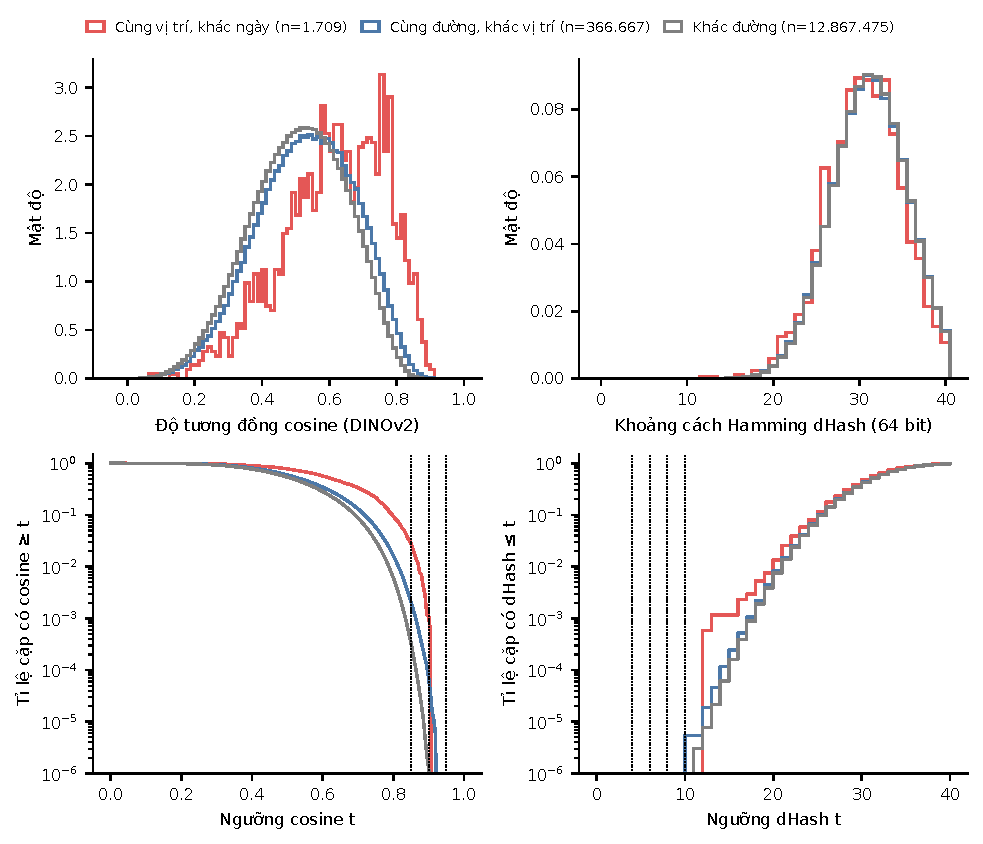
\includegraphics[width=0.92\textwidth]{dup_distance_distributions.pdf}
\caption{Phân bố độ tương đồng giữa các cặp ảnh: cùng vị trí khác ngày, cùng đường khác vị trí, khác đường}
\label{fig:dupdist}
\end{figure}

\subsubsection*{Rò rỉ giữa các tập}

Rò rỉ giữa các tập được đánh giá theo hai cách: theo nội dung ảnh và theo vị trí địa lý (hình~\ref{fig:map}).

\begin{figure}[H]
\centering
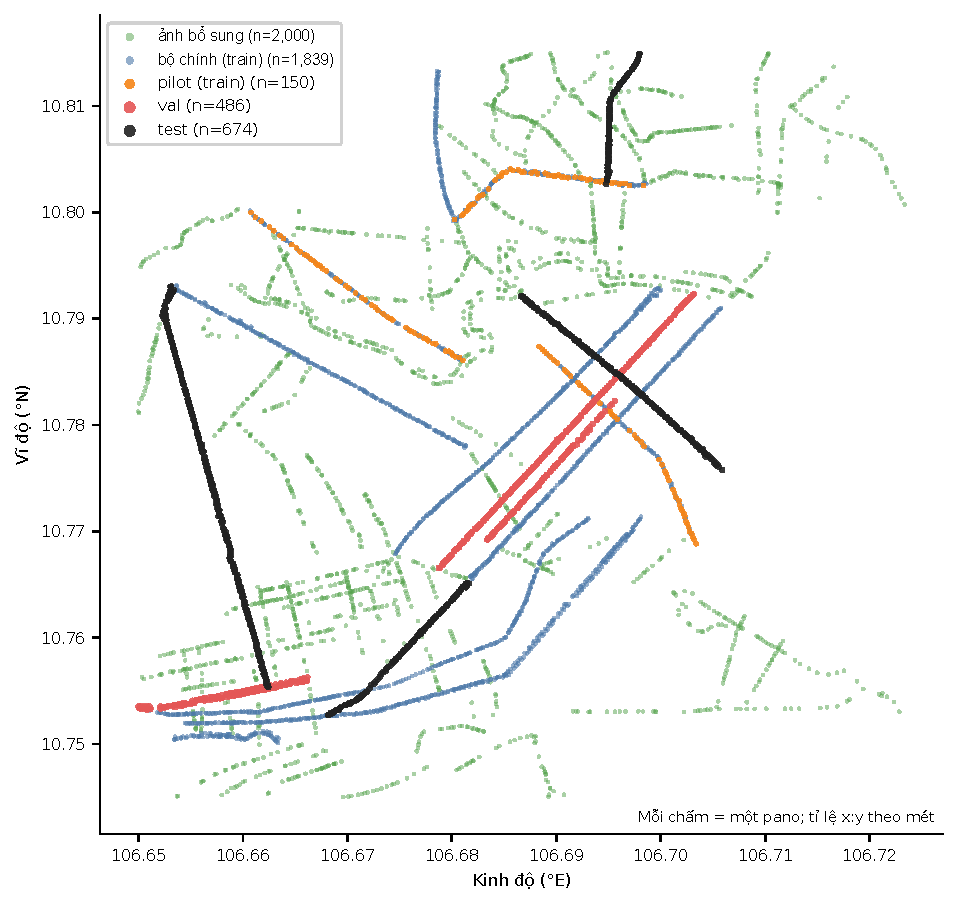
\includegraphics[width=0.8\textwidth]{dup_map_positions.pdf}
\caption{Vị trí của mọi ảnh theo tập. Các đường val/test cắt đường train tại giao lộ}
\label{fig:map}
\end{figure}

\textbf{Theo nội dung ảnh.} Với mỗi ảnh val/test, ảnh giống nhất ở phía train (bộ chính, pilot, ảnh bổ sung) được tìm theo độ tương đồng cosine.
\begin{itemize}
  \item Độ tương đồng với ảnh train gần nhất: val có trung vị 0,78, lớn nhất 0,909; test có trung vị 0,79, lớn nhất 0,904. Phân bố này trùng với mức tham chiếu giữa các đường train với nhau (trung vị 0,81, lớn nhất 0,933); nói cách khác, mức tương đồng giữa val/test và train không cao hơn mức tương đồng giữa hai đường train bất kỳ.
  \item Có 7 ảnh val/test có độ tương đồng cosine $\ge 0{,}90$ với một ảnh train, nhưng cả 7 cặp đều cách nhau 778--3.585 m. Kiểm tra trực quan 20 cặp giống nhau nhất cho thấy đều là hai địa điểm khác nhau có cùng kiểu cảnh (dãy nhà phố, người đi xe máy ở tiền cảnh).
\end{itemize}

\textbf{Theo vị trí địa lý.} Việc chia theo đường không ngăn được trường hợp đường val/test \emph{cắt} đường train tại giao lộ. Bảng~\ref{tab:spatial} thống kê số ảnh val/test nằm gần ảnh phía train.

\begin{table}[H]
\centering
\caption{Số ảnh val/test nằm gần một ảnh phía train}
\label{tab:spatial}
\begin{tabularx}{\textwidth}{>{\raggedright\arraybackslash}p{0.3\linewidth} R R R R R}
\toprule
\textbf{Cặp} & \textbf{Gần nhất (m)} & \textbf{< 15 m} & \textbf{< 25 m} & \textbf{< 40 m} & \textbf{< 100 m} \\
\midrule
Val (486) -- train bộ chính & 1,5 & 6 & 6 & 14 & 47 \\
Val -- pilot & 17,9 & 0 & 1 & 5 & 17 \\
Val -- ảnh bổ sung & 41,6 & 0 & 0 & 0 & 71 \\
Test (674) -- train bộ chính & 7,1 & 8 & 18 & 34 & 88 \\
Test -- pilot & 20,9 & 0 & 2 & 4 & 7 \\
Test -- ảnh bổ sung & 34,3 & 0 & 0 & 3 & 116 \\
\bottomrule
\end{tabularx}
\end{table}

\begin{itemize}
  \item \textbf{52 trên 1.160 ảnh val/test (4,5\%) nằm cách một ảnh train dưới 40 m}, liên quan tới 47 ảnh phía train và 13 cặp đường giao nhau (ví dụ Hồng Bàng -- Nguyễn Trãi, Lý Thường Kiệt -- Cách Mạng Tháng Tám, Hai Bà Trưng -- Điện Biên Phủ).
  \item Kiểm tra trực quan 20 cặp gần nhau nhất (1--14 m): phần lớn nhìn về hai hướng khác nhau, nhưng một số cặp thấy cùng một góc phố (cùng cột điện, biển quảng cáo, hàng rào). Phép đo theo nội dung không phát hiện được các cặp này: độ tương đồng cosine lớn nhất của chúng chỉ là 0,82.
  \item \textbf{Ảnh bổ sung tuân thủ quy tắc 40 m}, trừ 1 ảnh cách ảnh test 34,3 m (do quy tắc được áp dụng cho tâm của ô 25 m, không áp dụng cho từng ảnh).
  \item 53 trên 551 chuỗi ảnh Mapillary chứa ảnh của cả phía train lẫn val/test (cùng một lượt xe chạy qua nhiều đường). Đây không phải rò rỉ nội dung, nhưng cho thấy cùng một thiết bị và điều kiện chụp xuất hiện ở cả hai phía.
\end{itemize}

\textbf{Kế hoạch xử lý} (chưa thực hiện, cần nhóm quyết định trước khi khóa chia tập): loại khỏi train các ảnh cách ảnh val/test dưới 40 m, tương tự quy tắc đã áp dụng cho ảnh bổ sung. Quy tắc này chỉ dùng tọa độ, không dùng nhãn val/test, và loại tối đa 47 ảnh train. Phương án thay thế là giữ nguyên dữ liệu và báo cáo kết quả test kèm một lượt đánh giá loại bỏ 52 ảnh gần giao lộ.

\subsubsection*{Mức khác biệt giữa ảnh bổ sung và bộ chính}

Một bộ phân loại tuyến tính trên vector đặc trưng DINOv2, không dùng nhãn vật cản, được huấn luyện để phân biệt hai nhóm ảnh; AUC bằng 0,5 nghĩa là không phân biệt được. Việc đánh giá dùng xác thực chéo (cross-validation) chia theo đường. Bảng~\ref{tab:domain} trình bày kết quả; hình~\ref{fig:tsne} minh họa phân bố các vector đặc trưng bằng t-SNE.

\begin{figure}[H]
\centering
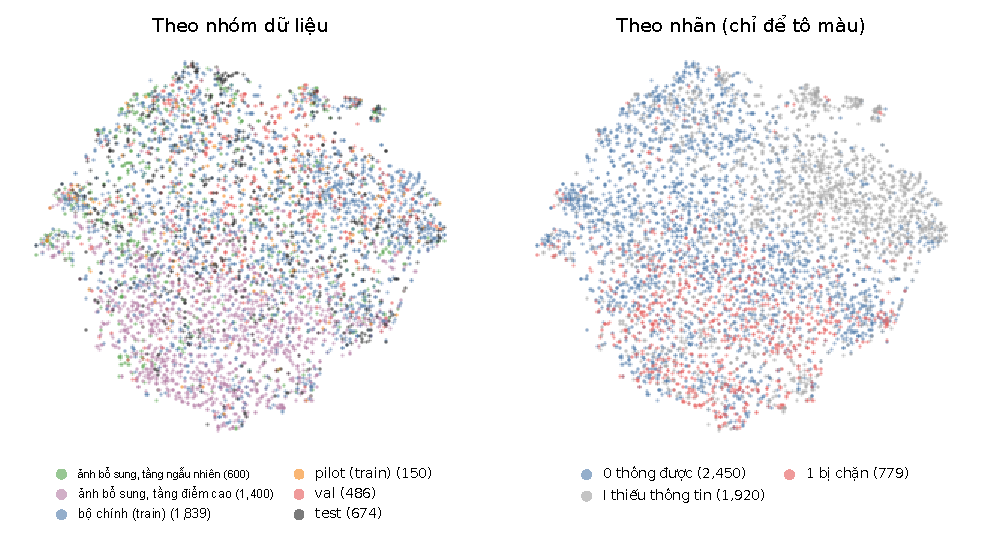
\includegraphics[width=\textwidth]{dup_tsne.pdf}
\caption[Hình chiếu t-SNE của embedding DINOv2 cho 5.149 ảnh, tô theo nhóm và theo nhãn]{Hình chiếu t-SNE~\cite{maaten2008tsne} của embedding DINOv2 cho 5.149 ảnh, tô màu theo nhóm và theo nhãn (nhãn chỉ dùng để tô màu)}
\label{fig:tsne}
\end{figure}

\begin{table}[H]
\centering
\caption{Mức phân biệt được giữa các nhóm ảnh (AUC của bộ phân loại miền)}
\label{tab:domain}
\begin{tabularx}{\textwidth}{>{\raggedright\arraybackslash}p{0.5\linewidth} R L}
\toprule
\textbf{So sánh} & \textbf{AUC} & \textbf{Diễn giải} \\
\midrule
Train bộ chính -- ảnh bổ sung, tầng điểm cao & 0,95 & Khác biệt rõ \\
Train bộ chính -- ảnh bổ sung, tầng ngẫu nhiên & 0,70 & Khác biệt vừa phải \\
Ảnh bổ sung -- val + test & 0,83 & Khác biệt rõ \\
Train bộ chính -- val + test & 0,47 & Không phân biệt được \\
Đối chứng: chia đôi ngẫu nhiên các đường train & 0,51 & Mức nền \\
\bottomrule
\end{tabularx}
\note{Trung bình qua các fold; độ lệch chuẩn giữa các fold 0,02--0,08.}
\end{table}

\begin{itemize}
  \item \textbf{Chưa phát hiện khác biệt miền ảnh giữa train bộ chính và val/test bằng bộ phân loại đã dùng} (AUC gần 0,5); tuy nhiên, kết quả này chưa chứng minh hai phân phối giống nhau. Với chỉ 17 đường, phép đo không đủ nhạy để phát hiện các khác biệt nhỏ.
  \item \textbf{Giá trị gộp 0,47 che khuất các giá trị dao động mạnh khi tách riêng:} train bộ chính so với val là 0,56, so với test là 0,36, so với pilot là 0,35 (trung bình qua các fold; độ lệch chuẩn giữa các fold tới 0,12). AUC dưới 0,5 ở đây không phải tín hiệu ngược chiều mà cho thấy phép đo không ổn định khi mỗi phía chỉ có vài đường.
  \item \textbf{Ảnh bổ sung thuộc một miền khác}, kể cả tầng ngẫu nhiên (0,70): các ảnh này đến từ những đường nhỏ gần chợ, trong khi val/test là các đường lớn. Tầng điểm cao còn đồng nhất hơn các nhóm khác (độ tương đồng cosine trung bình trong nhóm 0,60 so với 0,49--0,51). Đây là sự đánh đổi của việc bổ sung dữ liệu: có thêm 577 mẫu dương nhưng từ một dải cảnh hẹp hơn val/test.
  \item \textbf{Giá trị 0,95 của tầng điểm cao bị ước lượng cao một phần}: tầng này được chọn bằng hồi quy logistic trên chính các vector đặc trưng DINOv2 mà bộ phân loại miền sử dụng, nên một phần khả năng phân biệt đến từ chính cách chọn ảnh. Nhận xét này cũng áp dụng cho độ tương đồng cosine trong nhóm và hình t-SNE. Giá trị phản ánh khách quan hơn mức khác biệt về cảnh là của tầng ngẫu nhiên (0,70).
  \item Trên hình~\ref{fig:tsne}, ảnh \lab{Bị chặn} và ảnh tầng điểm cao tập trung về cùng một vùng, còn ảnh \lab{I} tập trung ở một vùng khác. Hình t-SNE chỉ dùng để minh họa, không dùng để rút ra kết luận.
\end{itemize}

\textbf{Trước khi khóa tập}, nhóm cần quyết định phương án xử lý theo khoảng cách địa lý, lưu manifest với phiên bản cố định và chạy lại các thống kê liên quan. Danh sách đường test được giữ nguyên, không thay đổi dựa trên số mẫu dương đã quan sát.


% ------------------------------------------------------------------------------
\subsection{EDA cho dữ liệu ảnh}
\label{sec:eda-image}

Mục này mô tả định dạng, độ phân giải và chất lượng ảnh theo từng nhóm, đồng thời xét mối liên hệ giữa chất lượng ảnh và nhãn. Hình~\ref{fig:examples} và hình~\ref{fig:examples-extra} minh họa ảnh của từng nhãn và từng tầng.

\begin{figure}[H]
\centering
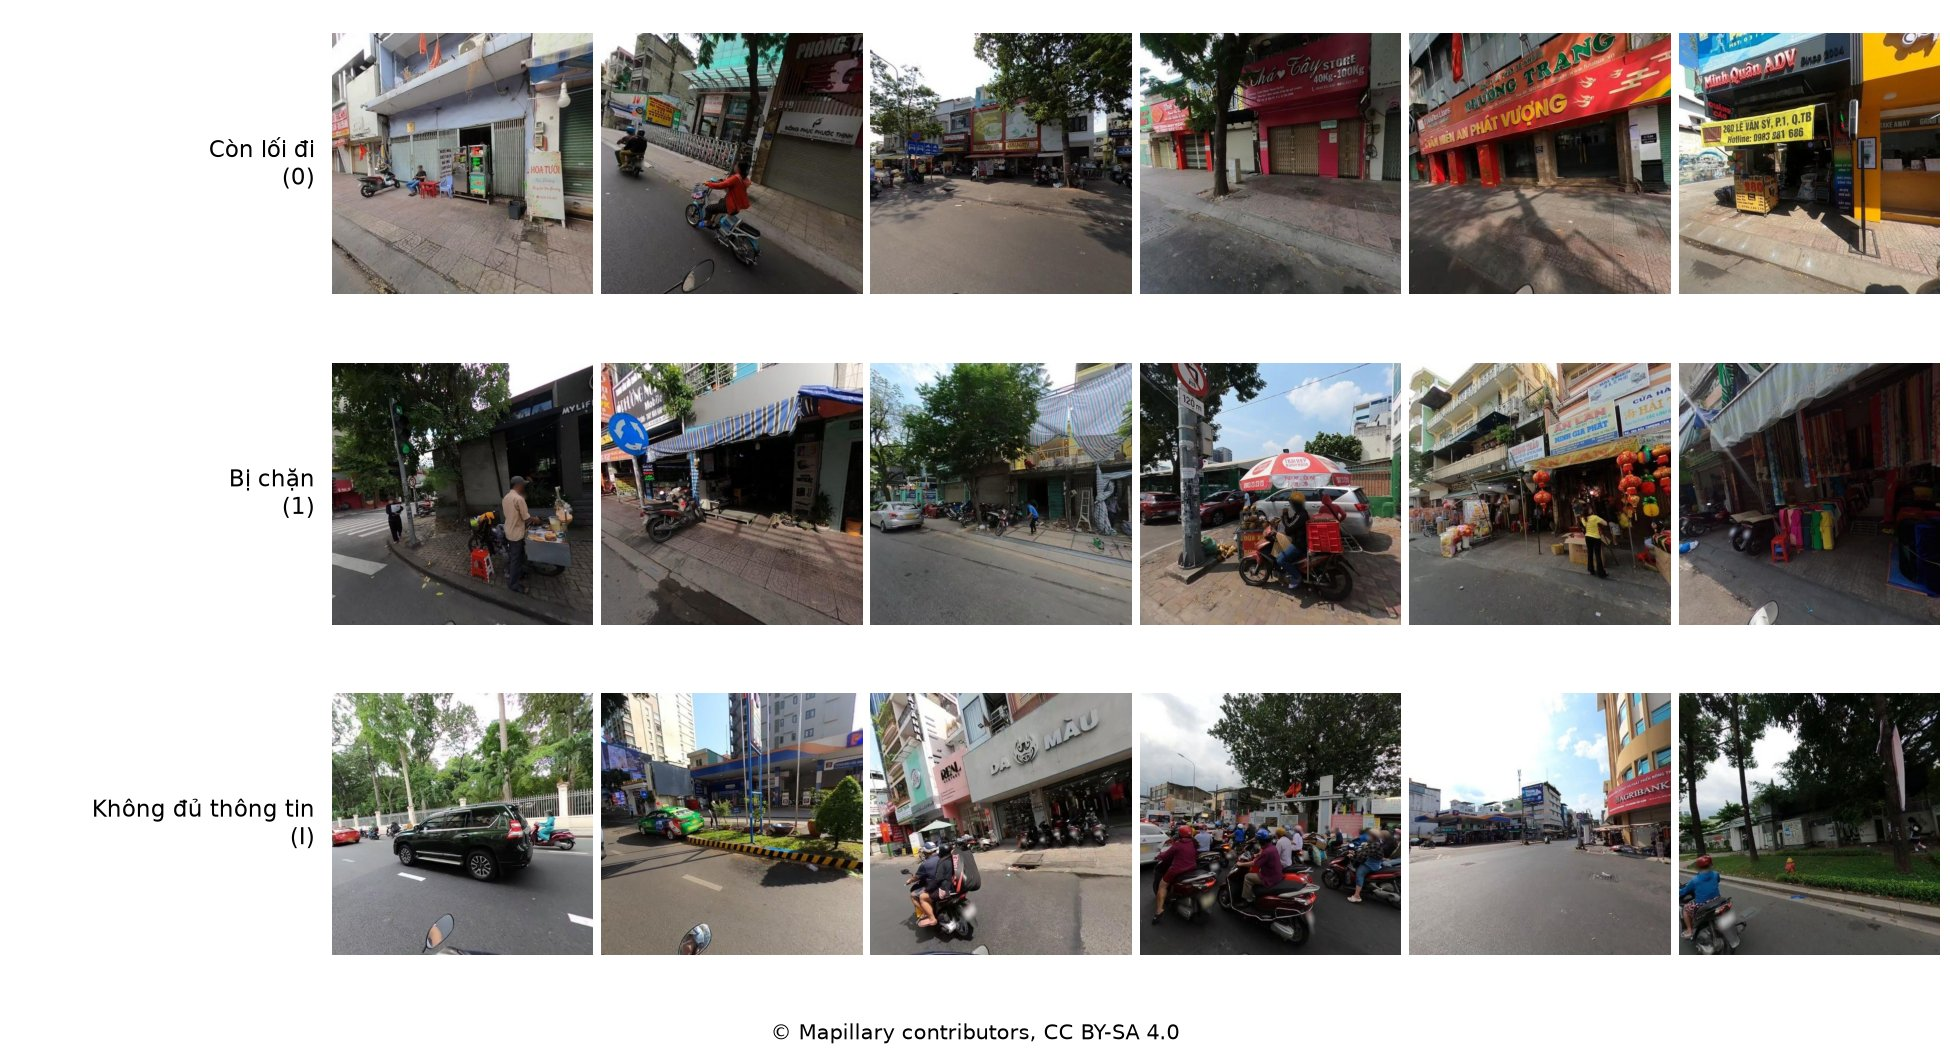
\includegraphics[width=\textwidth]{img_examples_main_train.jpg}
\caption{Ví dụ ảnh theo nhãn, lấy ngẫu nhiên từ train của bộ chính. \cc}
\label{fig:examples}
\end{figure}

\begin{figure}[H]
\centering
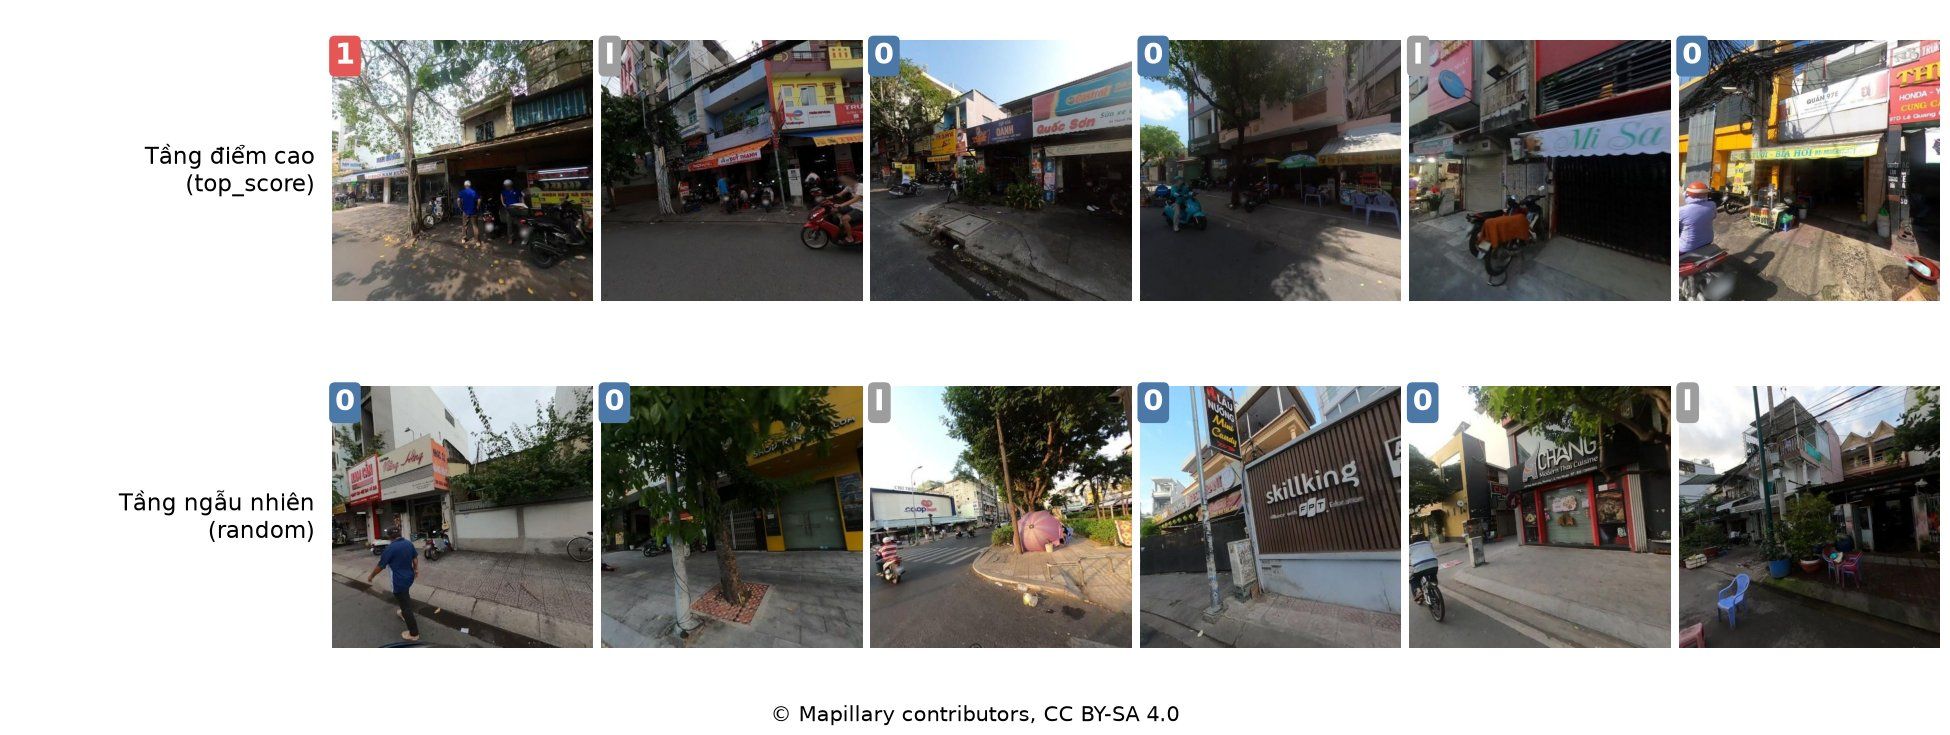
\includegraphics[width=\textwidth]{img_examples_train_extra.jpg}
\caption[Ví dụ ảnh bổ sung theo tầng lấy mẫu]{Ví dụ ảnh bổ sung theo tầng lấy mẫu; mỗi tầng gồm 6 ảnh lấy ngẫu nhiên nên tỉ lệ nhãn trong hình không đại diện cho tầng; ô góc trái ghi nhãn của ảnh. \cc}
\label{fig:examples-extra}
\end{figure}

\subsubsection*{Định dạng và độ phân giải}

Toàn bộ 5.149 ảnh đều đọc được, ở định dạng JPEG RGB $640\times640$ điểm ảnh, chất lượng nén ước lượng 90. Dung lượng mỗi ảnh từ 38,5 đến 167,7 KB, trung vị 99,3 KB. Độ phân giải đồng nhất theo thiết kế; do ảnh gốc là ảnh $360^\circ$ đã thu nhỏ còn 2.048 điểm ảnh, các chi tiết nhỏ ở xa bị mất.

\subsubsection*{Chất lượng ảnh}

Các đại lượng được đo trên từng ảnh cắt gồm: độ sáng trung bình (thang xám Rec.601, 0--255), độ tương phản (độ lệch chuẩn của thang xám), tỉ lệ điểm ảnh rất tối ($<30$) và cháy sáng ($>245$), độ nét (phương sai của toán tử Laplacian) và độ sặc sỡ màu~\cite{hasler2003colorfulness}.

\begin{table}[H]
\centering
\caption{Thống kê chất lượng ảnh theo nhóm (trung vị; trong ngoặc là IQR)}
\label{tab:image}
\begin{tabularx}{\textwidth}{>{\raggedright\arraybackslash}p{0.21\linewidth} r R R R R}
\toprule
\textbf{Nhóm} & \textbf{n} & \textbf{Độ sáng} & \textbf{Tương phản} & \textbf{Độ nét} & \textbf{Sặc sỡ màu} \\
\midrule
Bộ chính, train & 1.839 & 101,9 (31,3) & 59,4 (14,1) & 494 (254) & 25,1 (13,3) \\
Bộ chính, val & 486 & 106,7 (36,9) & 62,7 (14,1) & 560 (354) & 26,7 (13,7) \\
Bộ chính, test & 674 & 104,7 (36,9) & 59,3 (14,2) & 511 (245) & 25,9 (14,0) \\
Pilot & 150 & 106,6 (38,0) & 59,3 (14,0) & 487 (244) & 24,5 (13,1) \\
Ảnh bổ sung, tầng điểm cao & 1.400 & 91,8 (30,5) & 60,1 (13,7) & 492 (260) & 27,8 (14,3) \\
Ảnh bổ sung, tầng ngẫu nhiên & 600 & 100,8 (35,2) & 58,1 (12,4) & 497 (268) & 25,7 (13,7) \\
\midrule
Cả 5.149 ảnh: nhỏ nhất -- lớn nhất & & 24,3 -- 242,3 & 17,4 -- 96,6 & 22 -- 1.881 & 4,8 -- 104,3 \\
\bottomrule
\end{tabularx}
\end{table}

\begin{figure}[H]
\centering
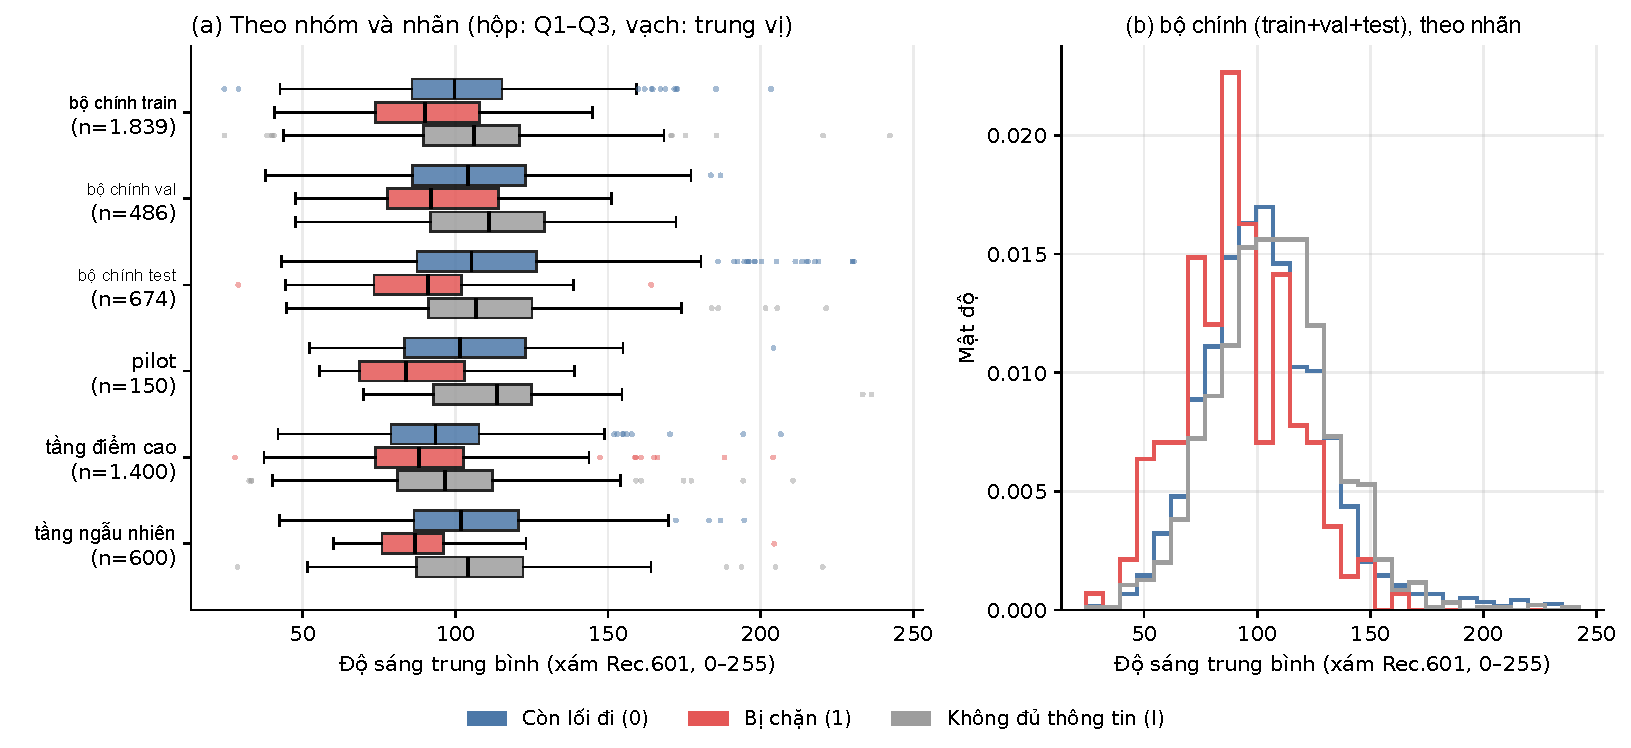
\includegraphics[width=\textwidth]{img_dist_luminance.pdf}
\caption{Độ sáng của ảnh cắt theo nhóm và theo nhãn}
\label{fig:lum}
\end{figure}

\begin{figure}[H]
\centering
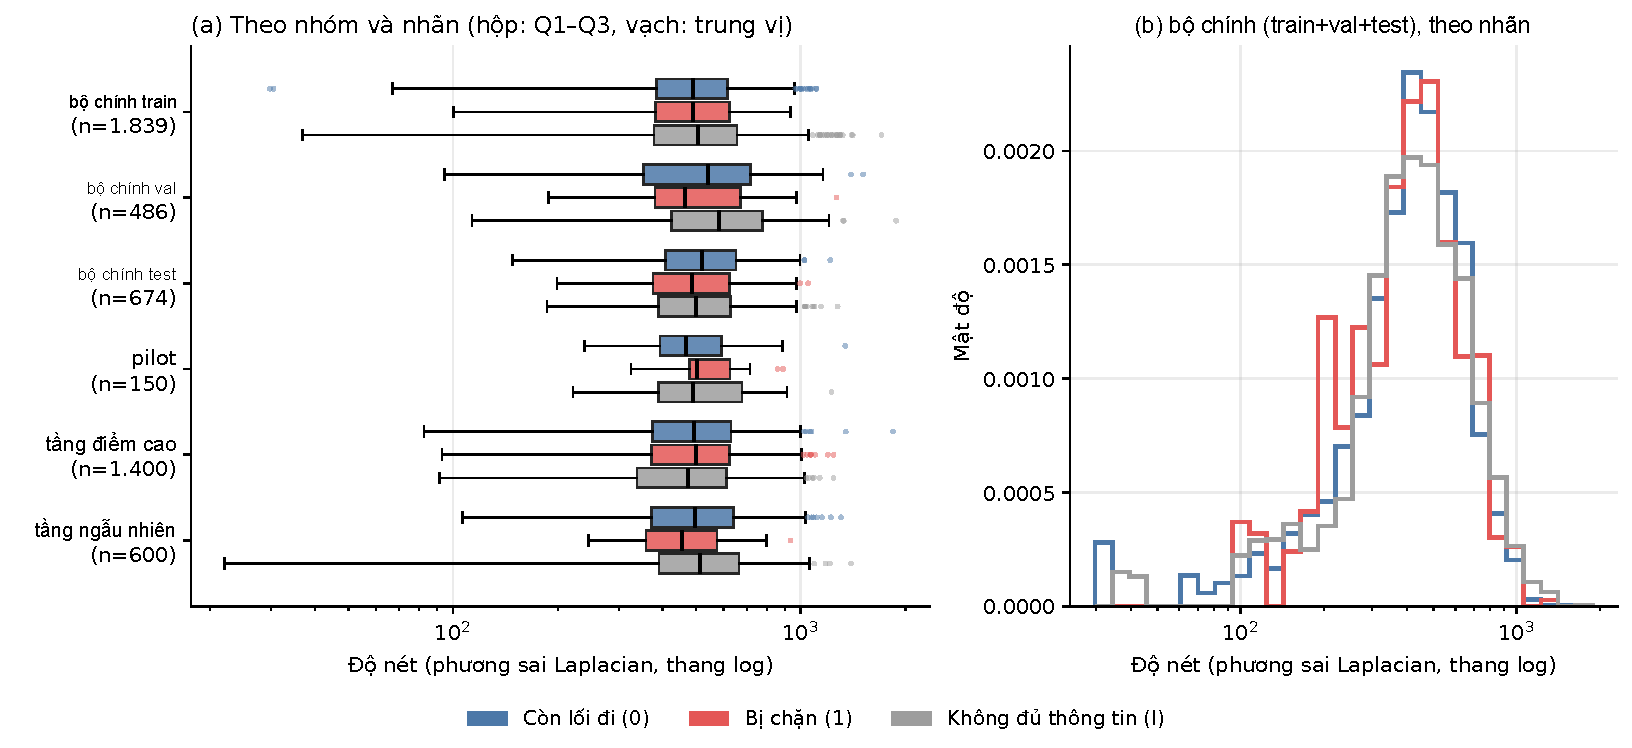
\includegraphics[width=\textwidth]{img_dist_sharpness.pdf}
\caption{Độ nét của ảnh cắt (thang log) theo nhóm và theo nhãn}
\label{fig:sharp}
\end{figure}

\begin{itemize}
  \item \textbf{Các nhóm tự nhiên có chất lượng ảnh tương đồng} (bảng~\ref{tab:image}, hình~\ref{fig:lum} và~\ref{fig:sharp}). Train, val, test, pilot và tầng ngẫu nhiên có trung vị độ sáng 101--107 và độ nét 487--560. Ảnh val có độ tương phản cao hơn train một chút (AUC 0,58 $[0{,}54;\,0{,}61]$).
  \item \textbf{Ảnh \lab{Bị chặn} tối hơn ảnh \lab{Còn lối đi}.} Ở bộ chính, trung vị độ sáng là 90,9 so với 101,6; AUC 0,37 $[0{,}32;\,0{,}41]$ (bootstrap theo 17 đường); tỉ lệ điểm ảnh rất tối là 18\% so với 12\%. Một cách giải thích hợp lý là vật cản thường nằm dưới mái hiên và bóng cây, nhưng giả thuyết này \textbf{chưa được kiểm chứng}. Đây là rủi ro học lối tắt: mô hình có thể dựa một phần vào độ tối của ảnh, nên cần kiểm tra khi phân tích lỗi mô hình.
  \item \textbf{Tầng điểm cao tối hơn bộ chính} (trung vị 91,8 so với 101,9), một phần vì tầng này có nhiều ảnh \lab{Bị chặn}.
  \item \textbf{Ảnh \lab{I} có độ tương phản cao hơn và nhiều vùng cháy sáng hơn} ảnh \lab{0} (AUC 0,67 và 0,65 ở bộ chính), phù hợp với việc các ảnh này thường chứa nhiều bầu trời và lòng đường.
  \item \textbf{Độ nét không phân biệt được \lab{Bị chặn} với \lab{Còn lối đi}} (AUC 0,46--0,59 ở mọi nhóm, mọi khoảng tin cậy đều chứa 0,5). Ở các so sánh có nhãn \lab{I}, hai khoảng tin cậy không chứa 0,5 nhưng hiệu ứng nhỏ: ở val, \lab{I} so với \lab{1} có AUC 0,61 $[0{,}53;\,0{,}71]$; ở tầng điểm cao, \lab{I} so với \lab{0} có AUC 0,46 $[0{,}42;\,0{,}49]$.
  \item \textbf{Độ sáng ảnh $360^\circ$ (dùng để lọc ảnh đêm) chỉ liên hệ yếu với độ sáng ảnh cắt} (Spearman 0,18 $[0{,}09;\,0{,}27]$ ở bộ chính; 0,31 nếu chỉ tính nửa trên ảnh cắt), vì hai đại lượng này đo hai vùng ảnh khác nhau. Do đó, bộ lọc ảnh đêm không bảo đảm ảnh cắt đủ sáng.
\end{itemize}

\subsubsection*{Đối chiếu lý do gán nhãn \lab{I} với phép đo chất lượng ảnh}

Có 33 ảnh \lab{I} mang lý do ``Ảnh mờ / tối / cháy sáng'' (bộ chính 12, ảnh bổ sung 21). Các ảnh này có độ nét thấp rõ rệt: trung vị độ nét nằm ở phân vị 3,5 của bộ chính và phân vị 13 của ảnh bổ sung. Về độ sáng, nhóm này gồm cả ảnh tối lẫn ảnh cháy sáng (36\% nằm dưới phân vị 10, 18\% nằm trên phân vị 90). Do cỡ mẫu nhỏ, kết quả này chỉ mang tính mô tả.
